\documentclass[10pt]{article}
\usepackage[T1]{fontenc}
\usepackage{lmodern,amsmath,amssymb,graphicx,hyperref}
\usepackage[margin=.74in]{geometry}
\setlength{\parindent}{0pt}\setlength{\parskip}{7pt}
\begin{document}
\begin{center}{\Large Materialized arithmetic-event counts}\\[4pt]
Local successor --- 15 November 2026\end{center}
\textbf{Working result.} Draft034 locally elaborates177 theorem statements,
including previous local work, with exit0/no warnings. Printed central
expression-value, multiplication-event and actual coefficient/cast-bound
lists use standard foundations. Primitive calls now supply an event trace;
the complete materialized expression's multiplication count equals the
previously declared scalarProducts model. This is local evidence, outside
Transport53/shared57/fresh. All data are unsigned/defaultnot\_covered
[pcc:unverified].

\textbf{Events at calls.} A scalar multiplication returns its product and a
multiply event; addition returns its sum and an add event. The explicit
list dot loop invokes those primitives, recursively evaluates the remaining
pairs, and concatenates their emitted traces. The count is not a desired
recurrence attached to the result. Its returned value is the exact dot
product, and each multiply/add count equals the pair-list length
[pcc:unverified].

For stored child vectors and coefficient$(b,n)$, build pairs by flattening
the two antidiagonals. Their cardinality is derived from the actual finite
lists:
\[
 |\{(i,j):i+j=b\}|\,|\{(r,s):r+s=n\}|=(b+1)(n+1).
\]
Thus the logged coefficient returns the actual convolution value and exactly
$(b+1)(n+1)$ multiplication events and the same number of addition events.
Zero contributions still execute the declared operations; no sparse-output
or constant-time shortcut is assumed [pcc:unverified].

\textbf{Whole stored boxes.} Materialize logged coefficient cells in core
Vectors, map their values into a result Vector, and flatten the emitted
traces. The trace count is the actual sum of cell trace counts. A whole
$h\times z$ convolution therefore emits
\[
 P(h,z)=\sum_{b<h}\sum_{n<z}(b+1)(n+1)
\]
multiplication events and the same number of addition events. Its value
agrees with the earlier stored-box multiplication. The equality follows
from traversal/cardinality proofs, not from coefficient value equality alone
[pcc:unverified].

Expression evaluation first builds its stored children, then invokes logged
materialized addition, negation or convolution. A literal is cast once before
its array is built and emits a cast event. The returned values agree with
full polynomial coefficients and with the earlier stored evaluator; for the
actual Packed approximation this retains the previous canonical-value
interface at creation precision [pcc:unverified].

\textbf{Exact evidence.} Single-coefficient local160 data PCC-20261115-bbd1dc;
whole-box local167 data9c9ee4; expression local177 dataa634cb (same prefix).
Receipts015--017 retain failed029/031/033 and accepted030/032/034 source,
raw compiler output and exits. No new independent shared-gate/fresh coverage.

\newpage
\begin{center}{\Large Count-model equality and remaining bit-cost obligations}\end{center}
For expression$e$, define$Q_{h,z}(e)$ recursively: leaves cost0;
addition sums child costs; negation preserves child cost; multiplication
sums child costs and adds$P(h,z)$. The new event-bearing interpreter derives
\[
 \#\mathrm{multiply}(\mathrm{traceEval}(e))=Q_{h,z}(e).
\]
If$C(e)$ counts literal leaves, it also derives
\[
 \#\mathrm{cast}(\mathrm{traceEval}(e))=C(e)
 \le\mathrm{nodes}(e).
\]
These statements concern emitted scalar-call events. They do not identify
events with machine steps or integer bit operations [pcc:unverified].

For the actual Packed approximation, let$M=\sum_{j<u}m_j$ and retain the
previous proved node bound
\[
 N_*=1+(17+20\cdot2^a+13M+2u)
       +(29+10M+2u)(k+1)^2.
\]
With$h=b+1,z=n+1$, the actual logged coefficient has bounds
\[
 \#\mathrm{multiply}\le N_*\bigl((b+1)(n+1)\bigr)^2,
 \qquad \#\mathrm{cast}\le N_*.
\]
Unary powers, grid cardinality and all mask multiplicities remain in the
node bound. Every$2^u k$ label remains charged. These are per-coefficient
approximation-pass bounds; outer right scaling, denominator preparation and
finite extraction are not silently included [pcc:unverified].

\begin{center}
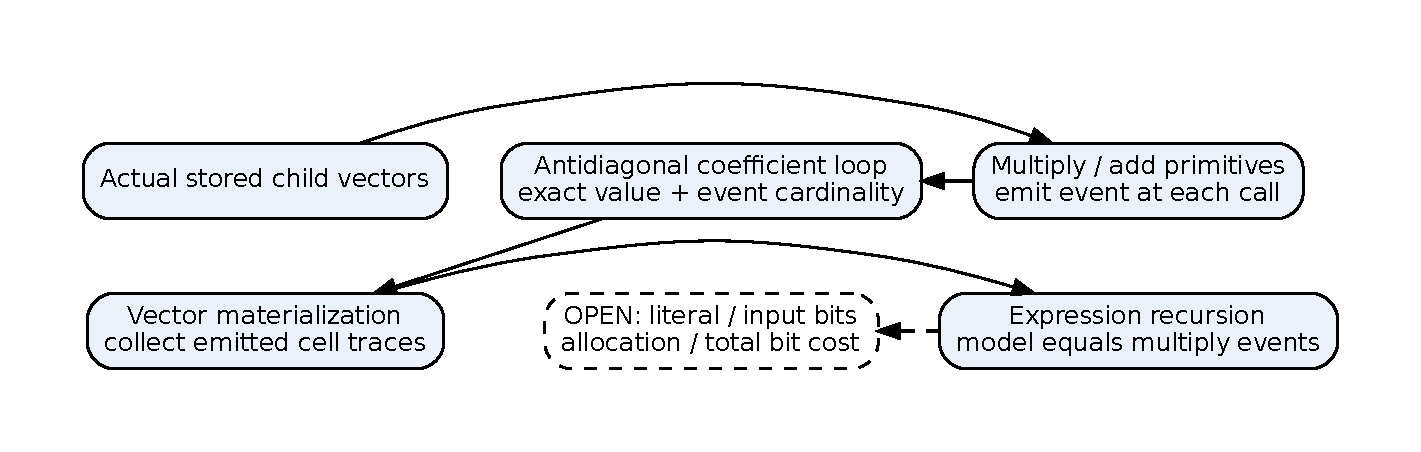
\includegraphics[width=\linewidth,height=1.6in,keepaspectratio]{events-dependencies-001.pdf}
\end{center}

\textbf{Next exact obligation.} Derive a Packed budget invariant controlling
positive denominator and every integer literal from the actual rational
scalar Bits results. Propagate through arithmetic, products, unary powers
and geometric clearing, including empty products and$k=0$. Then price input
and expression construction, normalization, enumeration/sorting, indexing,
array allocation, trace/logging overhead, modular arithmetic/inversion,
retained memory and total integer bit cost. Event-list append itself has
uncharged overhead; no linear-time or free-erasure assumption is made
[pcc:unverified].

\textbf{Scope and sources.} Standard primitive-event semantics, exact list
count/flatMap sums, antidiagonal cardinality, core Vector Basic/OfFn/Lemmas,
Fin.sum\_ofFn and Finset.sum\_range. KB unavailable as logged; no novelty,
measured speed or tested extracted executable claim. All older archive86/48
and source/evidence/claims remain exact at their historical scopes. Original
creation, modes, children, recursion and public expected-cost bridges stay
separate. No paid/cloud/native attack/fixture or timing campaign
[pcc:unverified].
\end{document}
